\kapitola{Návrh řešení}
Tato kapitola obsahuje návrh řešení založený na požadavcích identifikovaných v předchozí kapitole. Na základě těchto požadavků byl návrh rozdělen do dvou projektů a to webového frontendu, který slouží jako rozhraní ukazující průběh simulace realném čase a serverové části, která slouží pro rychlý výpočet simulace bez vykreslovaní na platformě Node.js.

Jelikož obě části budou používat stejný simulační kód bylo rozhodnuto, že bude samotná simulace vytvořena jako softwarová knihovna. Tuto závislost ilustruje obrázek \ref{fig:dependency}.
\begin{figure}[h!]
	\centering
	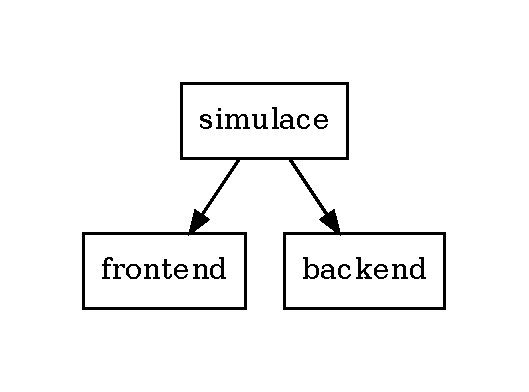
\includegraphics[width=0.4\linewidth]{architektura}
	\caption{Schéma závislostí}
	\label{fig:dependency}
\end{figure}


\sekce{Simulace}
Z obrázku \ref{fig:dependency} je zřejmé, že simulační kód spojuje obě části dohromady. Je tedy důležité, aby byl navržený tak, aby jej bylo co nejjednodušeji integrovat s oběma řešeními.

Na základě těchto požadavků a podmínek, které jsou stanoveny v předchozí kapitole byl vytvořen následující návrh:

\label{sec:ECS}
Simulace je navržena v duchu ECS (\textbf{Entity component system}) podrobný popis lze nalézt v sekci \ref{sec:ces}. Není tedy žádným překvapením, že se všechny komponenty nalezené v simulaci dají rozložit na systémy, komponenty a entity. Pro lepší představu o implementaci je níže uveden přehled všech systému, entit a komponent použitých v simulaci.

\podsekce{Diagram tříd}
Níže popsaný návrh doplňuje diagram tříd, který zobrazuje jejích návaznost a zároveň také do návrhu zavádí třídu \textbf{Simulation}, která celou simulaci schovává za jednoduché rozhraní a umožňuje snadnou integraci simulace do různých aplikací.

\begin{figure}[H]
	\centering
 	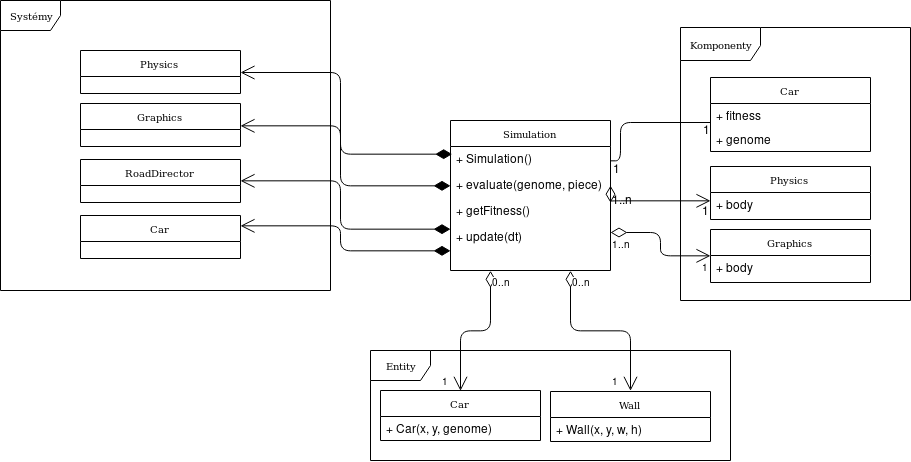
\includegraphics[width=0.7\linewidth]{classDiagram}
	\caption{Diagram tříd}
	\label{fig:class-diagram}
\end{figure}

\podsekce{Entity}
Simulace obsahuje následující entity:

\textbf{PhysicsGroup} Seskupuje fyzikální entity do jedné pro snadnou manipulaci s nimi.

\textbf{RoadPart} Entita, která obaluje jednu nebo více překážek tak, aby se s nimi dalo snadno pohybovat používá se pro tvorbu složitějších dílů vozovky.

\textbf{Car} Reprezentuje samotné vozidlo obsahuje jak jeho grafickou reprezentaci, tak kompletní logiku a fyzikální model.

\podsekce{Komponenty}
Simulace obsahuje následující komponenty:
\begin{itemize}
	\item \textbf{Car} obsahuje všechny potřebné informace o agentovi. Toto zahrnuje vše od neurnové sítě, která je použitá pro jeho řízení po ovládání jednotlivých kol agenta.
	\item \textbf{Graphics} komponenta, která obsahuje grafické informace pro \textbf{Pixi.js}.
	\item \textbf{Physics} komponent, která obsahuje fyzikální entity pro \textbf{P2.js}
\end{itemize}

\podsekce{Systémy}
Návrh simulace obsahuje následující systémy:

\textbf{Car} systém, který se stará o ovládání agenta a částečně o vyhodnocování jeho fitness.

\textbf{Graphics} grafický systém, který slouží především k překreslování entit.

\textbf{Physics} krokuje fyzikální engine a synchronizuje grafickou reprezentaci s fyzikální entitou. Tento proces probíhá pro každý snímek a skládá se z přiřazení nové rotace a pozice pro grafickou entitu.

\textbf{RoadDirector} Road director se stará o generování nekonečného prostředí pro agenta. Děje se tak na základě předefinovaných dílu vozovky z nichž každý zaplňuje celou obrazovku simulace. V případě, že agent dorazí až na konec obrazovky je mu určen nový navazující dílek. Agent je pak přehozen na opačnou stranu obrazovky a zároveň je vyměněn díl na kterém se nachází.
Hlavní výhodou tohoto přístupu je to, že agent může jezdit po vozovce donekonečna bez starosti o to, že by se dostal na limit fyzikálního enginu (přetečení pozice fyzikálního objektu). Další nesporná výhoda tohoto přístupu je úspora paměťových nároků, kterou by s sebou nesla definice větší mapy a možnost generování náhodných map pro testování agenta.

\podsekce{Fitness funkce}
Fitness funkce je důležitou součástí simulace, která zásadně ovlivňuje chování výsledných agentů a je tedy nutné jí volit vhodně. Je nutné, aby funkce agenta motivovala ke správné činnosti.

Po několika pokusech a konzultaci s vedoucím práce byla jako metrika úspěchu agenta zvolena celková vzdálenost, kterou je agent schopný překonat v průběhu jedné generace. Výpočet je realizován s pomocí RoadDirectoru, který si při každém přechodu zaznamená bod, ve kterém se po přesunu agent nachází. Výsledná fitness je pak součet uražených vzdáleností pro každou místnost. Road direktor si pro každou obrazovku uchovává vzdálenost, kterou agent v dané obrazovce překonal. Výsledným fitness je pak součet všech vzdáleností na všech obrazovkách.

\sekce{Klientská část}
Klientská část je webové rozhraní, které vzniklo z požadavků na vizualizaci a ověření funkčnosti simulační knihovny. 

Z požadavků vyšla aplikace, která obsahuje 3 rozdílné obrazovky a to jedne, která slouží pro zobrazení a simulaci vývoje algoritmu v reálném čase. Další slouží pro zpětné přehrávání již vygenerovaných genomů a poslední obrazovka, která umožňuje uživateli vyzkoušet ovládat agenta.

\sekce{Serverová část}
Serverová část byla nakonec navržena a vytvořena ve dvou na sebe navazujících verzích. 

\podsekce{První verze}
Je ilustrovaná na obrázku \ref{fig:server_first}. Návrh první verze popisuje jednoduchou aplikaci, která rozkládá vyhodnocování jednotlivých genomů mezi jednoho nebo více zpracovatelů. Každý zpracovatel běží ve vlastním vlákně a zátěž je tedy rozložena mezi dostupná jádra procesoru. Zpracovatel po vyhodnocení genomu vrací hlavnímu vláknu fitness daného jedince. Ten si ho uloží a po vyhodnocení všech jedinců tímto způsobem provede algoritmus NEAT. Tento proces se opakuje do té doby, než nedojde k naplnění ukončujících podmínek (maximální počet generací) nebo přerušení programu.

\begin{figure}[H]
	\centering
	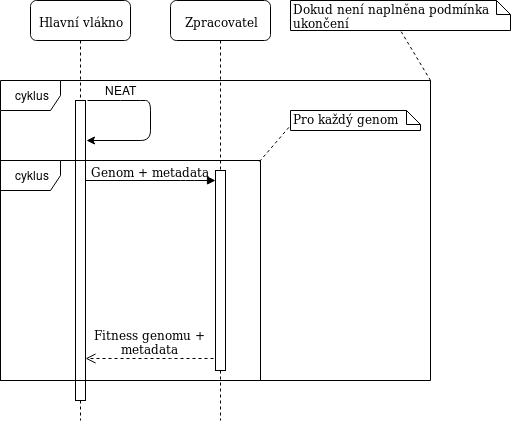
\includegraphics[width=0.7\linewidth]{server_first_use_case}
	\caption{První verze serverové části}
	\label{fig:server_first}
\end{figure}

\podsekce{Druhá verze}
Druhá verze rozšiřuje návrh o možnost rozložení výpočtů mezi více počítačů. Byla navržená poté, co bylo zjištěno, že předchozí verze nebyla schopná vyhodnotit dostatečné množství genomů dostatečně rychle.

Pracuje dle diagramu \ref{fig:distributed}, kde je vidět, že klient zadává do fronty úkoly (genom a nastavení simulace). Jednotliví zpracovatelé (počítače v~clusteru), kteří si je z~ní vyberou, jednotlivé genomy vyhodnotí a hodnotu fitness funkce pošlou zpět na klienta. Toto je ilustrováno v diagramu \ref{fig:serverusecase}.

\begin{figure}[H]
	\centering
	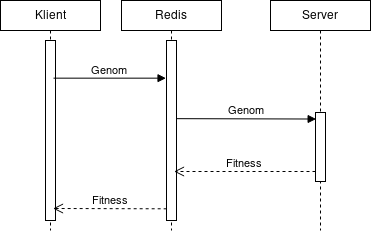
\includegraphics[width=0.7\linewidth]{server_use_case}
	\caption{Sekvenční diagram komunikace se serverem}
	\label{fig:serverusecase}
\end{figure}

Jakmile klient dostane všechny hodnoty zpět provede na populaci algoritmus NEAT (mutace, křížení, \dots) a poté je nová generace poslána znovu na vyhodnocení.

\podsekce{Databáze}
Všechny verze serverové části zaznamenávají průběh algoritmu NEAT do databáze jejíž schéma lze vidět v obrázku \ref{fig:database}. Databáze obsahuje tabulku \textbf{Genomes}, která uchová fitness nejlepšího a nejhoršího jedince v generaci, zároveň také obsahuje nejlepší genom z dané generace. Každý záznam v tabulace \textbf{Genomes} má přidělenou konfiguraci se kterou byl spuštěn. Toto je důležité při vyhodnocování více konfigurací zároveň, které je popsáno níže.

\begin{figure}[H]
	\centering
	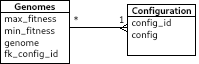
\includegraphics[width=0.7\linewidth]{ERD}
	\caption{Schéma databáze}
	\label{fig:database}
\end{figure}

\sekce{Fitness funkce}
\label{sec:fitness}

Agenta je ovšem kromě motivace třeba také penalizovat za akce, které jsou nepřípustné. V případě simulace se jedná především o kolizi s překážkou, za což je agent penalizován předčasným ukončením simulace a nemožností tedy zvýšit svoji fitness.

\sekce{Agent}
Definice agenta zásadně ovlivňuje výsledek simulace, protože stanovuje vstupy a výstupy do a z~neuronové sítě. V této práci je testováno několik konfigurací, které jsou popsány níže.

V případě této práce je agentem auto, které je vybaveno vzdálenostními senzory. Měření těchto senzorů je normalizováno (maximální vzdálenost měřícího paprsku je 800 m) a předáno jako vstup do neuronové sítě.

Agent bude testován v různých konfiguracích: 


\podsekce{Řízení agenta}

Řízení agenta probíhá tak, že se každý snímek s~pomocí neuronové sítě na obrázku \ref{fig:control_network} rozhoduje, jakou akci podnikne. Má následující možnosti:

\begin{enumerate}
	\item Ovládání volantu 
	\begin{enumerate}
		\item $z_1$ Otočení volantem o určitý počet stupňů doleva
		\item $z_2$ Otočení volantem o určitý počet stupňů doprava
	\end{enumerate} 
	\item Rychlostní stupně
	\begin{enumerate}
		\item $z_3$ - zpátečka
		\item $z_4 - z_6$ - rychlosti dopředu
	\end{enumerate}
\end{enumerate}

Ovládání volantu i volba rychlostního stupňů probíhá zároveň a to tak, že se vždy z dané skupiny neuronů vybere ten, který má největší hodnotu. Tento přístup je identický tomu, který se používá například u neuronových sítí pro klasifikaci.

\begin{figure}[H]
	\centering
	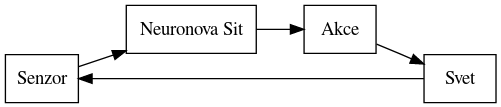
\includegraphics[width=0.7\linewidth]{AgentSchema}
	\caption{Řízení agenta}
	\label{fig:agentschema}
\end{figure}

%digraph { 
%	rankdir=LR
%	graph [ nodesep=0.5] 
%	node [shape=box] 
%	"Senzor" -> "Agent"
%	"Agent" -> "Akce"
%	"Akce" -> "Svet"
%	"Svet" -> "Senzor"
%}

\begin{figure}[H]
	\centering
	\begin{neuralnetwork}[height=7]
		\newcommand{\nodetextx}[2]{\ifthenelse{\equal{#2}{0}}{$b_0$}{$s_{#2}$}}
		\newcommand{\nodetextz}[2]{$z_#2$}
		\newcommand{\nodetexth}[2]{\ifthenelse{\equal{#2}{0}}{$b_1$}{$h_{#2}$}}
		\inputlayer[count=6, title={Data ze senzorů}, text=\nodetextx]
		\hiddenlayer[count=6, title={Skrytá vrstva}]
		\linklayers
		\outputlayer[count=6, title={Výstup}, text=\nodetextz] 
		\linklayers
	\end{neuralnetwork}
	\caption{Neuronová síť agenta}
	\label{fig:control_network}
\end{figure}

\podsekce{Možné konfigurace agenta} 
Výše uvedenou konfiguraci lze rozšířit o níže uvedené vstupy/výstupy.

Modifikace vstupů umožní agentovi vnímat více než jen vzdálenosti z jednotlivých senzorů. Bude zajímavé pozorovat, jak se agent s jednotlivými vjemy poradí. V práci se vyzkouší následující přidané vstupy:
\begin{itemize}
	\item aktuální rychlost
	\item náklon volantu
\end{itemize}

Modifikovat lze také výstupy neuronové sítě toto rozšíří nebo omezí možnosti agenta:
\begin{itemize}
	\item Přidáním/odebráním možnosti brzdění
	\item Přidáním/odebráním možnosti udržení volantu ve stejné pozici
	\item Modifikací možností rychlostí a to:
	\begin{itemize}
		\item Foo
	\end{itemize}
\end{itemize}
%- na vstup site privest i aktualni rychlost a natoceni volantu (to co
%ridic prece v kabine vidi, kdyz auto ridi)
%- mozna bych zrusil jednotlive rychlostni stupne, nechal bych jen
%zpatecku/brzdu a jizdu dopredu/akceleraci (tzn. jeden neuron je
%akcelerace a druhy brzda nebo couvani)
